\documentclass{ltjsarticle}
\usepackage{amsmath}
\usepackage{amssymb}
\usepackage{ascmac}
\usepackage[dvipdfmx]{graphicx}
\usepackage{tabularx}
\usepackage[colorlinks=true, allcolors=blue]{hyperref}
\usepackage{fancybox}
\usepackage{tikz}
\usepackage{subcaption}
\usetikzlibrary{shapes,arrows}

\begin{document}

\title{105. 深層学習の適用方法(GAN)}
\author{秋葉洋哉}
\maketitle

\section{GAN}
\subsection{概要}
GAN(Generative Adversarial Networks)は、生成モデルの一つであり、生成モデルは、データの分布を推定し、新しいデータを生成するためのモデルである。GANは、生成器(Generator)と識別器(Discriminator)の2つのネットワークを用いて学習を行う。ある分布$p_z$をGenerator $G$に入力したときの出力$p_g$を、Discriminator $D$に入力する。すると、$D$は、$p_g$が$p_z$から生成されたデータであるか、実際のデータであるかを判定する。$G$は、$D$が$p_g$を実際のデータと誤認識するように学習し、$D$は、$G$が生成したデータを実際のデータと区別するように学習する。このように、$G$と$D$が互いに学習することで、生成モデルを学習することができる。
\par
この2者は、ゼロサムゲームの関係にある。つまり、$G$が勝つ確率と$D$が勝つ確率の和は1になる。$G$は、$D$が$p_g$を実際のデータと誤認識する確率を最小化し、$D$は、$G$が生成したデータを実際のデータと区別する確率を最小化することを目指す。
\begin{itemize}
  \item $G$ : 相手が勝利する確率を最小化する作戦を取る
  \item $D$ : 自分の勝利する確率を最大化する作戦を取る
\end{itemize}
\par
これを数式で表すと、以下のようになる。
\begin{align}
  &\min_G \max_D V(D, G) \\
  \label{eq:V_GAN}
  &\text{s.t. } V(D, G) = \mathbb{E}_{x \sim p_{data}(x)}[\log D(x)] + \mathbb{E}_{z \sim p_z(z)}[\log(1 - D(G(z)))]
\end{align}
ただし、$V(D, G)$は、$D$と$G$のゲームの価値関数であり、$p_{data}(x)$は、実際のデータの分布、$p_z(z)$は、生成器に入力するノイズの分布である。また、$x$は、実際のデータ、$z$は、ノイズである。また、$\mathbb{E}$は、期待値を表す。
\par
生成データが本物のようなデータを生成するのはなぜだろうか。
以下では、$p_g = p_{data}$であると仮定したときに、価値関数が最適化されていることを示す。
まず、Generatorの出力がすべて真のデータであったとする。すると、$V$は以下のように展開できる。
\begin{align}
  V(D, G) &= \mathbb{E}_{x \sim p_{data}(x)}[\log D(x)] + \mathbb{E}_{z \sim p_z(z)}[\log(1 - D(x))]\\
  &= \int_x p_{data}(x) \log D(x) dx + \int_z p_z(z) \log(1 - D(x)) dz\\
  &= \int_x \left( p_{data}{(x)} \log D(x) + p_g(x) \log(1 - D(x)) \right) dx\\
  &= \int_x a\log(y) + b\log(1 - y) dx
\end{align}
ただし、$a = p_{data}(x)$、$b = p_g(x)$、$y = D(x)$と置いた。この時の極大値は、
\begin{align}
  \frac{\partial V}{\partial y} &= \frac{a}{y} - \frac{b}{1 - y} = 0\\
  \therefore y &= \frac{a}{a + b} \\
  &= \frac{p_{data}(x)}{p_{data}(x) + p_g(x)}
\end{align}
となる。この条件を満たすとき、$V$は最大値を取る。
さらに、価値関数の$D(x)$を$\frac{p_{data}(x)}{p_{data}(x) + p_g(x)}$に置き換えると、
\begin{align}
  V(D, G) &= \mathbb{E}_{x \sim p_{data}(x)}[\log D(x)] + \mathbb{E}_{z \sim p_z(z)}[\log(1 - D(G(z)))]\\
  &= \mathbb{E}_{x \sim p_{data}(x)}\log\left[ \frac{p_{data}(x)}{p_{data}(x) + p_g(x)} \right] + \mathbb{E}_{x \sim p_g(x)}\log\left[ \frac{p_g(x)}{p_{data}(x) + p_g(x)} \right]\\
  &= \mathbb{E}_{x \sim p_{data}(x)}\log\left[ \frac{2p_{data}(x)}{p_{data}(x) + p_g(x)} \right] + \mathbb{E}_{x \sim p_g(x)}\log\left[ \frac{2p_g(x)}{p_{data}(x) + p_g(x)} \right] - 2\log 2\\
  &= 2JS(p_{data}||p_g) - 2\log 2
\end{align}
ただし、$JS$は、ジェンセン・シャノンダイバージェンスであり、$JS$が最小となるとき、$p_{data}(x) = p_g(x)$となる。
つまり、この価値関数に従うことで、$p_{data}(x)= p_g(x)$となる時に、最適解となることがわかる。
\par
ここで、クロスエントロピー誤差関数について思い出してみると、クロスエントロピー誤差関数は、
\begin{align}
  L = -y \log p - (1 - y) \log (1 - p)
\end{align}
で表せた。ただし、$y$は、正解ラベル、$p$は、予測値である。
例えば、真のデータを$p$に入力するときは、$y = 1$となり、$p = D(x)$が入力される。この時、$L = -\log D(x)$となる。また、Generator によって生成されたデータを$p$に入力するときは、$y = 0$となり、$p = D(G(z))$が入力される。この時、$L = -\log(1 - D(G(z)))$となる。
これらの2つの$L$を足し合わると
\begin{align}
  L = -\log D(x) - \log(1 - D(G(z)))
\end{align}
となる。これは単一のデータの場合の式\eqref{eq:V_GAN}と等価である。
つまり、GANの学習は、クロスエントロピー誤差関数の期待値を用いて、$D$と$G$の学習を行っていくことになる。

\subsection{GANの学習}
GANの学習は、以下の手順で行う。
\begin{enumerate}
  \item Generatorのパラメータ$\theta_g$を固定し、真のデータと生成データをm個ずつ取り出す。
  \item Discriminatorのパラメータ$\theta_d$を勾配上昇法で更新する。
  \item Discriminatorのパラメータ$\theta_d$を固定し、生成データをm個取り出す。
  \item Generatorのパラメータ$\theta_g$を勾配降下法で更新する。
\end{enumerate}
それぞれの更新式は以下で表せる。
\begin{align}
  \theta_d &\leftarrow \theta_d + \alpha \nabla_{\theta_d} \frac{1}{m} \sum_{i=1}^{m} \left[ \log D(x^{(i)}) + \log(1 - D(G(z^{(i)}))) \right] \\
  \theta_g &\leftarrow \theta_g - \alpha \nabla_{\theta_g} \frac{1}{m} \sum_{i=1}^{m} \log(1 - D(G(z^{(i)})))
\end{align}
ただし、$\alpha$は、学習率である。
GANでは、$\theta_d$をk回更新し、$\theta_g$を1回更新することが一般的である。

GANの学習過程を図\ref{fig:GAN}に示す。
\begin{figure}[htbp]
  \centering
  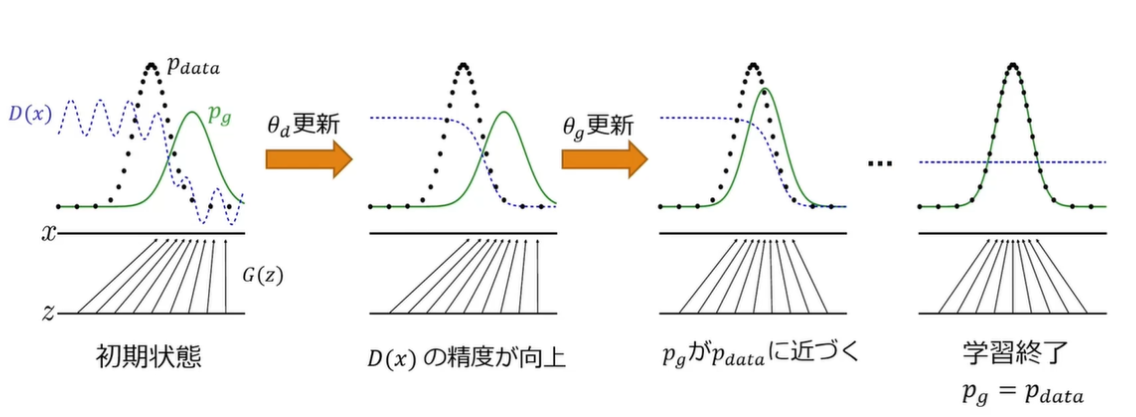
\includegraphics[width=13cm]{./capture/GAN.png}
  \caption{GANの学習過程}
  \label{fig:GAN}
\end{figure}

\begin{itembox}{}
  Discriminatorの実装例
  \begin{verbatim}
    cross_entropy = tf.keras.losses.BinaaryCrossentropy(from_logits=True)
    def discriminator_loss(real_output, fake_output):
      # 本物の画像に対するDiscriminatorの予測を1の配列と比較
      real_loss = cross_entropy(tf.ones_like(real_output), real_output)
      # 生成された画像に対するDiscriminatorの予測を0の配列と比較
      fake_loss = cross_entropy(tf.zeros_like(fake_output), fake_output)
      total_loss = real_loss + fake_loss
      return total_loss

  \end{verbatim}
\end{itembox}

\clearpage
\section{DCGAN}
\subsection{概要}
DCGAN(Deep Convolutional Generative Adversarial Networks)は、GANの一種であり、CNN(Convolutional Neural Networks)を用いて画像生成を行うモデルである。DCGANは、以下の構造制約を設けることで、生成品質を向上させることができる。
\begin{itemize}
  \item Generator : Pooling層の代わりに、転置畳み込み層(Transposed Convolutional Layer)を用いるを用い、最終層にtanh, 他の層にReLUを用いる。
  \item Discriminator : Pooling層の代わりに、畳み込み層を用い、最終層にSigmoid, 他の層にLeakyReLUを用いる。
  \item 共通事項 : 中間層に全結合層を用いず、Batch Normalizationを用いる。
\end{itemize}

\begin{figure}[htbp]
  \centering
  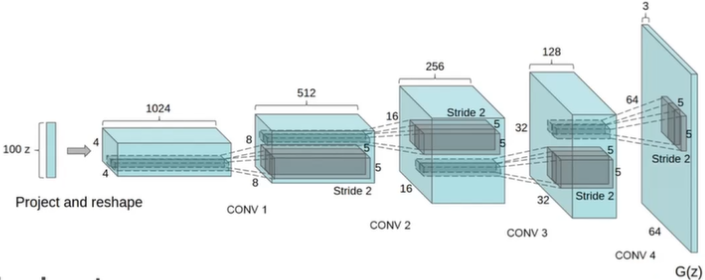
\includegraphics[width=13cm]{./capture/DCGAN.png}
  \caption{DCGANの構造: 乱数を与えると、4×4×1024の画像を生成し、そのチャンネル数を減らして縦横を増やしていくことで、64×64×3のRGB画像を出力する。}
  \label{fig:DCGAN}
\end{figure}

\subsection{Fast Bi-layer Neural Synthesis of One-Shot Realistic Head Avatars}
Zakharov et al. (2020)では、DCGANを用いて、1枚の顔画像から、顔の動画(Avatar)を高速で生成するモデルを提案した。
この論文では、初期化部と推論部から顔アバターを生成するモデルを提案した。
初期化では、人物の特徴を抽出し、1アバターにつき1回だけ実行される。推論部では、初期化部で生成された特徴を元に、所望の動きを付ける。時間フレームの分だけ推論部が実行され、動画が生成される。
従来のモデルと比較すると、初期化の計算コストを大きくして、推論部の計算コストを削減することで、高速でアバターを生成することができるようになった。
\par
推論部では、緻密な輪郭と荒い顔画像を別々に生成して結合することで、高速にアバターを生成することができるようになった。
\begin{figure}[htbp]
  \centering
  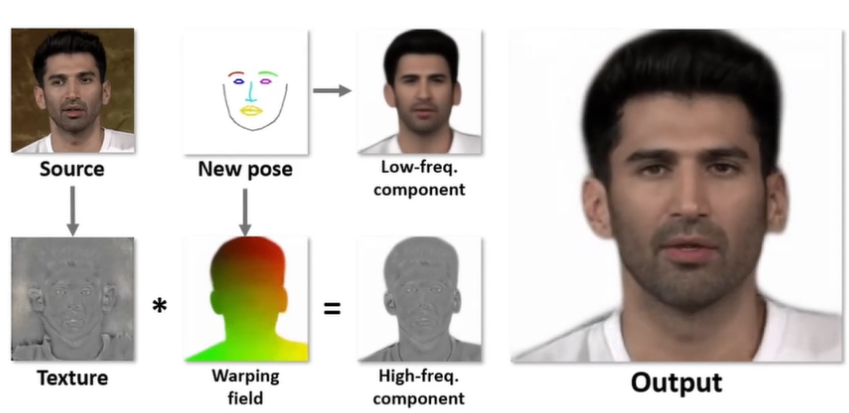
\includegraphics[width=13cm]{./capture/Avatar.png}
  \caption{Avatarの生成過程}
  \label{fig:Avatar}
\end{figure}

\begin{figure}[htbp]
  \centering
  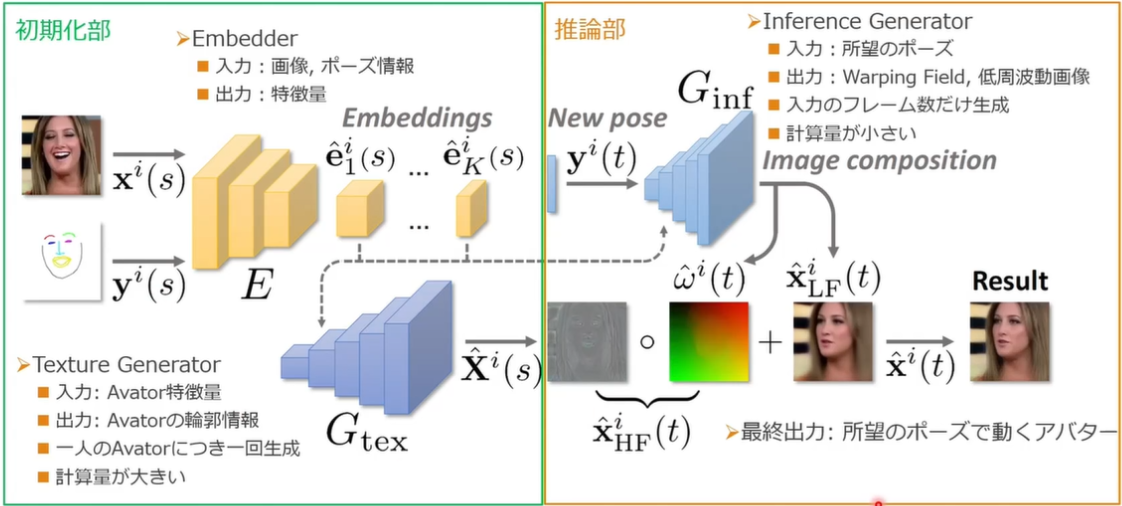
\includegraphics[width=13cm]{./capture/Avatar_Structure.png}
  \caption{Avatarの生成過程}
  \label{fig:Avatar2}
\end{figure}

\clearpage
\section{CGAN(conditional GAN)}
\subsection{概要}
CGAN(conditional GAN)は、条件付き生成モデルであり、生成器に条件パラメータを与えることで、GANでは指定できなかった生成したい画像のクラスを指定できる。CGANの損失関数は、以下のように表せる。
\begin{align}
  \min_G \max_D V(D, G) = \mathbb{E}_{x \sim p_{data}(x)}[\log D(x|y)] + \mathbb{E}_{z \sim p_z(z)}[\log(1 - D(G(z|y)))]
\end{align}
ただし、$y$は、条件である。
例えば、犬、という条件を与えると、Generatorは犬の画像を生成することができる。
一方、Discriminatorは、生成された画像かどうか、とその画像がラベルのクラスに分類されるかどうか、の2条件を判別する。その組み合わせの通りは、以下のようになる。
\begin{itemize}
  \item Gが生成した犬の画像 かつ ラベルが犬 と識別した場合→ 不正解
  \item Gが生成した犬の画像 かつ ラベルが犬以外 と識別した場合→ 不正解
  \item 真の犬の画像 かつ ラベルが犬 と識別した場合→ 正解
  \item 真の犬の画像 かつ ラベルが犬以外 と識別した場合→ 不正解
\end{itemize}
\begin{figure}[htbp]
  \centering
  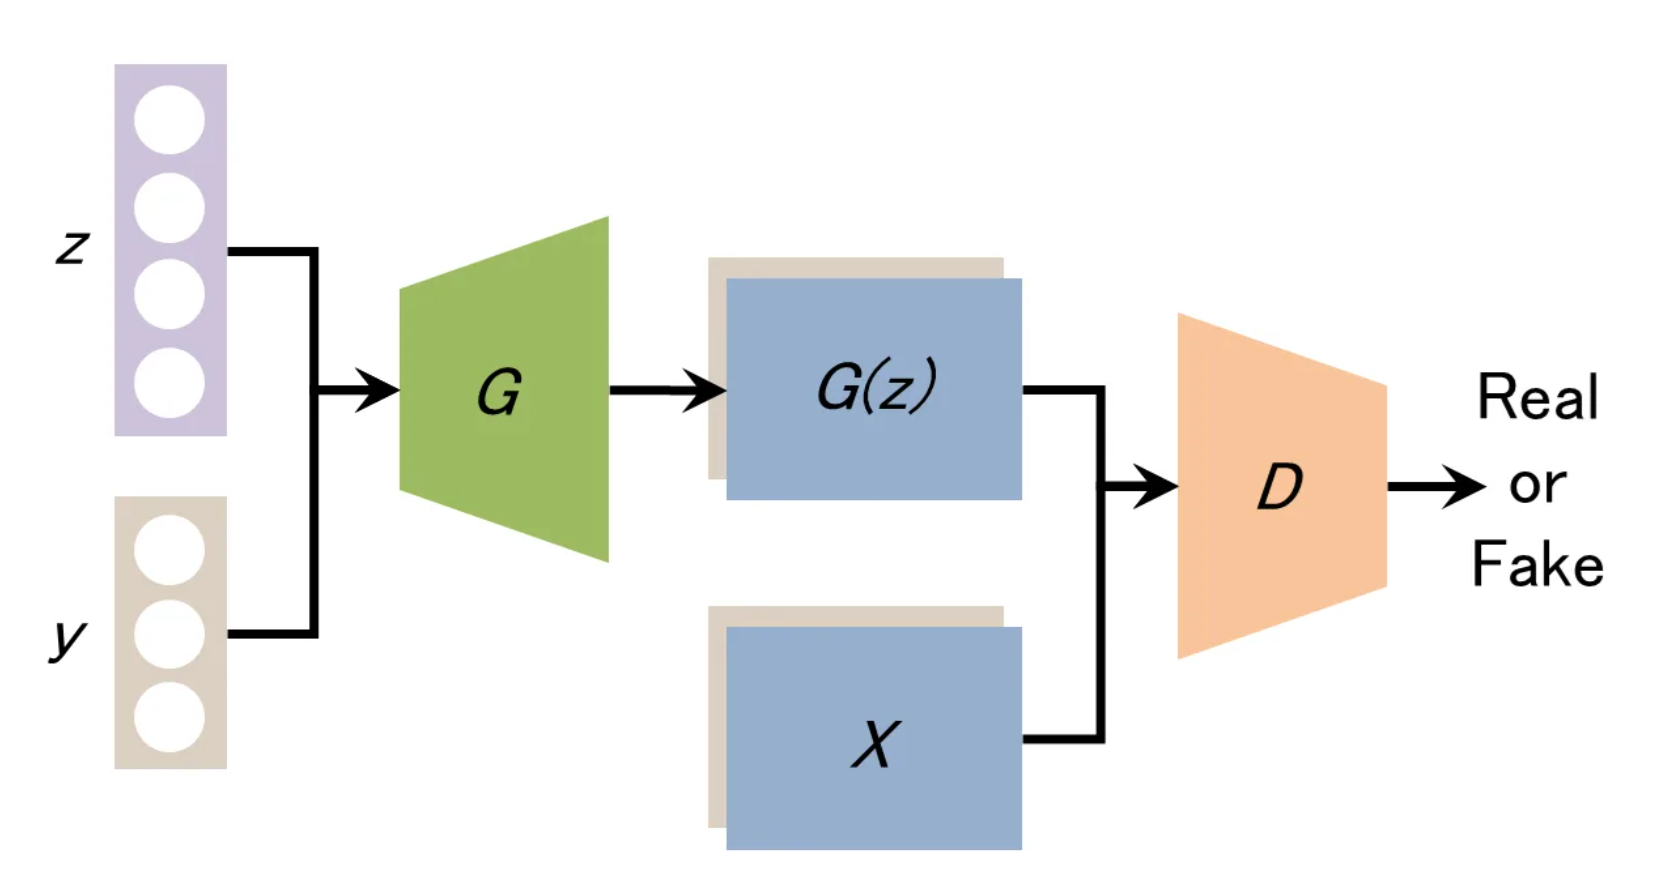
\includegraphics[width=13cm]{./capture/CGAN.png}
  \caption{CGANの構成}
  \label{fig:conditional_GAN}
\end{figure}

\paragraph{参考文献}
\begin{enumerate}
  \item 岡谷貴之/深層学習 改訂第2版 [機械学習プロフェッショナルシリーズ]/ 講談社サイエンティフィク/ 2022-01-17
  \item 深層畳み込み敵対的生成ネットワーク(DCGAN)\url{https://www.tensorflow.org/tutorials/generative/dcgan?hl=ja}
  \item CGAN (Conditional GAN):条件付き敵対的生成ネットワーク NegativeMindException \url{https://blog.negativemind.com/2019/10/05/conditional-gan/}
  \item Github @garridoq/gan-guide \url{https://github.com/garridoq/gan-guide}
\end{enumerate}

\clearpage
\section{実装演習キャプチャ}
%------------
%GAN
%------------
\subsection{GAN}
\begin{figure}[htbp]
  \centering
  \includegraphics[width=10cm]{C:/Users/hiroh/Videos/Captures/4_10_code_dcgan/Arc 2024_07_10 0_17_27.png}
\end{figure}
\begin{figure}[htbp]
  \centering
  \includegraphics[width=10cm]{C:/Users/hiroh/Videos/Captures/4_10_code_dcgan/Arc 2024_07_10 0_17_35.png}
\end{figure}
\begin{figure}[htbp]
  \centering
  \includegraphics[width=10cm]{C:/Users/hiroh/Videos/Captures/4_10_code_dcgan/Arc 2024_07_10 0_17_40.png}
  \caption{(コードはうまく回ったが、うまく生成できなかった。)}
\end{figure}
\end{document}